% =====================================================================
% Parte 02 — Gráficas de funciones (Stewart, Precálculo 7.ª ed., §2.2)
% Páginas del libro 159–169 (PDF 180–190, offset +21).
%
% Ejercicios elegidos (15), todos del bloque de ejercicios de §2.2:
%   Ej  4  (p. 167) — Conceptos: relacionar función con su gráfica
%   Ej  9  (p. 167) — 5–28 Trazar gráficas por tabla de valores
%   Ej 15  (p. 167) — 5–28 Trazar gráficas por tabla de valores
%   Ej 19  (p. 167) — 5–28 Trazar gráficas por tabla de valores
%   Ej 21  (p. 167) — 5–28 Trazar gráficas por tabla de valores
%   Ej 27  (p. 167) — 23–28 Valor absoluto
%   Ej 35  (p. 167) — 33–46 Funciones definidas por tramos
%   Ej 45  (p. 168) — 33–46 Funciones definidas por tramos
%   Ej 49  (p. 168) — 49–50 Fórmula a partir de la gráfica
%   Ej 51  (p. 168) — 51–52 Prueba de la recta vertical
%   Ej 55  (p. 168) — 53–56 Recta vertical: dominio y rango
%   Ej 57  (p. 168) — 57–68 Ecuaciones que definen funciones
%   Ej 61  (p. 168) — 57–68 Ecuaciones que definen funciones
%   Ej 81  (p. 169) — Aplicaciones (tarifas eléctricas)
%   Ej 83  (p. 169) — Aplicaciones (tarifas postales)
%
% Figuras recortadas del libro:
%   fig_p02_04.png (p. 167), fig_p02_49.png, fig_p02_51.png, fig_p02_55.png (p. 168)
% =====================================================================
\documentclass[11pt]{article}
\usepackage[utf8]{inputenc}
\usepackage[spanish]{babel}
\usepackage[margin=2.3cm]{geometry}
\usepackage{amsmath,amssymb}
\usepackage{enumitem}
\usepackage{tcolorbox}
\tcbuselibrary{skins,breakable}
\usepackage{pgfplots}
\pgfplotsset{compat=1.18}
\usepackage{tikz}
\usepackage{graphicx}
\usepackage{array}
\usepackage[hidelinks]{hyperref}

% Notación española opcional (descomenta si quieres \sen en lugar de \sin)
% \DeclareMathOperator{\sen}{sen}
% \DeclareMathOperator{\tg}{tg}
% \DeclareMathOperator{\ctg}{ctg}

\newtcolorbox{sol}{colback=blue!5,colframe=blue!50!black,title=Solución paso a paso,breakable}
\newtcolorbox{teo}{colback=orange!8,colframe=orange!70!black,title=Teoría,breakable}
\newtcolorbox{nota}{colback=green!5,colframe=green!50!black,title=Idea clave,breakable}
\newtcolorbox{tip}{colback=yellow!10,colframe=yellow!60!black,title=Consejo,breakable}
\newtcolorbox{resp}{colback=red!5,colframe=red!50!black,title=Respuesta,breakable}
\newtcolorbox{reg}{colback=red!5,colframe=red!60!black,title=Regla,breakable}
\newtcolorbox{paso}[1]{colback=gray!5,colframe=gray!50!black,title={#1},breakable}

\graphicspath{{../images/}{images/}}
\newcommand{\sen}{\operatorname{sen}}

% babel spanish activa < y > y rompe TikZ/pgfplots (->, >=stealth)
\AtBeginDocument{\shorthandoff{<>}}

% Corchetes dobles de la funcion mayor entero (Stewart), sin tocar preamble.tex
\newcommand{\ment}[1]{[\![#1]\!]}
\begin{document}

\section*{Parte 02 — Gráficas de funciones (Stewart §2.2, pp. 159--169)}

\begin{teo}
\textbf{Método de la sección 2.2.}
\begin{enumerate}[leftmargin=*]
\item \textbf{Gráfica de $f$:} es el conjunto $\{(x,f(x)) \mid x\in A\}$, con $A$ el dominio. Trazar $f$ es trazar la ecuación $y=f(x)$.
\item \textbf{Tabla de valores:} se eligen varios $x$ del dominio, se calcula $f(x)$, se colocan los puntos $(x,f(x))$ y se unen con una curva suave.
\item \textbf{Catálogo básico:} $f(x)=mx+b$ (recta), $f(x)=x^n$ (potencia), $f(x)=\sqrt[n]{x}$ (raíz), $f(x)=1/x^n$ (recíproca), $f(x)=|x|$ (V), $f(x)=\ment{x}$ (mayor entero). Reconocerlos evita tabular de cero.
\item \textbf{Funciones por tramos:} se traza cada fórmula \emph{solo} sobre su parte del dominio; punto sólido si el extremo se incluye, punto hueco si se excluye.
\item \textbf{Prueba de la recta vertical:} una curva del plano es gráfica de una función si y sólo si ninguna recta vertical la corta más de una vez.
\item \textbf{Ecuaciones que definen funciones:} se despeja $y$. Si el despeje da \emph{un} valor de $y$ por cada $x$, la ecuación define a $y$ como función de $x$; si da dos (típicamente por un $\pm\sqrt{\;}$), no.
\end{enumerate}
\end{teo}

\begin{tip}
Fórmulas que se repiten en toda la parte:
\[
|u|=\begin{cases}u & \text{si } u\ge 0\\ -u & \text{si } u<0\end{cases}
\qquad
\ment{x}=\text{mayor entero menor o igual a } x
\]
\[
\sqrt{u}\ \text{exige } u\ge 0,
\qquad
\frac{1}{u}\ \text{exige } u\ne 0,
\qquad
y^2=k\ (k>0)\ \Longrightarrow\ y=\pm\sqrt{k}.
\]
El $\pm$ es exactamente lo que rompe la definición de función: dos salidas para una entrada.
\end{tip}

% =====================================================================
\subsection*{Ejercicio 1 — Relacionar cada función básica con su gráfica (Ej.~4, p.~167)}

\begin{quote}
\textbf{4.} Relacione la función con su gráfica.

\quad \textit{a}) $f(x)=x^2$ \hfill \textit{b}) $f(x)=x^3$

\quad \textit{c}) $f(x)=\sqrt{x}$ \hfill \textit{d}) $f(x)=|x|$
\end{quote}

\begin{center}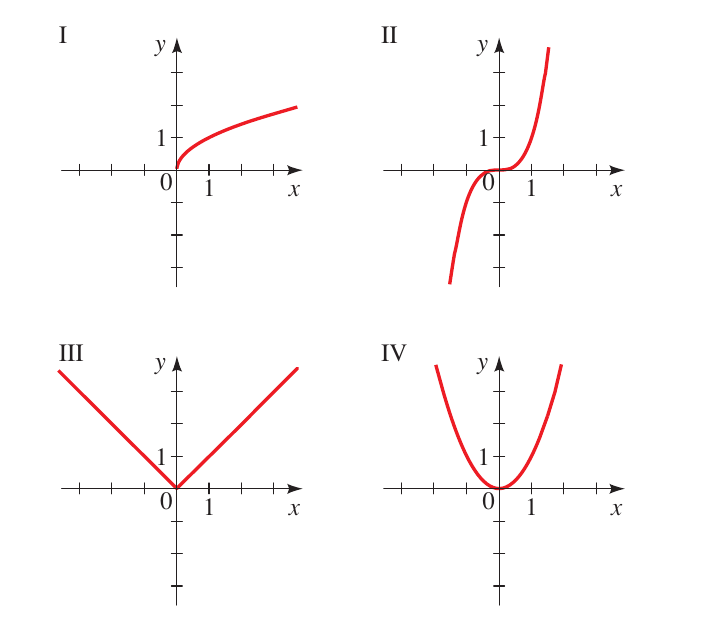
\includegraphics[width=0.62\textwidth]{fig_p02_04.png}\end{center}

\begin{paso}{Paso 1 --- Separo por dominio}
\textbf{Qué hago:} miro cuál gráfica vive sólo en $x\ge 0$.

\textbf{¿De dónde sale?} De las cuatro fórmulas, sólo $\sqrt{x}$ tiene dominio restringido.

\textbf{¿Por qué?} La raíz de índice par exige radicando no negativo, así que $\sqrt{x}$ existe únicamente para $x\ge 0$. La gráfica I es la única que no aparece a la izquierda del eje $y$: $c)\to \mathrm{I}$.
\end{paso}

\begin{paso}{Paso 2 --- Separo por paridad (simetría)}
\textbf{Qué hago:} evalúo $f(-x)$ en las tres restantes.

\textbf{¿De dónde sale?} $(-x)^2=x^2$ y $|-x|=|x|$ (pares, simétricas respecto al eje $y$); $(-x)^3=-x^3$ (impar, simétrica respecto al origen).

\textbf{¿Por qué?} Por la definición de función par e impar. La gráfica II es la única con simetría respecto al origen (baja a la izquierda y sube a la derecha): $b)\to \mathrm{II}$.
\end{paso}

\begin{paso}{Paso 3 --- Distingo $|x|$ de $x^2$ por la forma en el origen}
\textbf{Qué hago:} comparo las dos gráficas pares restantes, III y IV.

\textbf{¿De dónde sale?} $|x|$ coincide con las rectas $y=x$ y $y=-x$, así que su gráfica es una V de lados rectos con pico en $(0,0)$; $x^2$ es una parábola de lados curvos.

\textbf{¿Por qué?} Por la definición por tramos del valor absoluto (figura 7 del texto). III tiene lados rectos y IV es curva: $d)\to \mathrm{III}$ y $a)\to \mathrm{IV}$.
\end{paso}

\begin{resp}
$a)\ f(x)=x^2 \to \mathrm{IV}$; \quad $b)\ f(x)=x^3 \to \mathrm{II}$; \quad $c)\ f(x)=\sqrt{x} \to \mathrm{I}$; \quad $d)\ f(x)=|x| \to \mathrm{III}$.
\end{resp}

% =====================================================================
\subsection*{Ejercicio 2 — Gráfica de $f(x)=-x^2$ (Ej.~9, p.~167)}

\begin{quote}
\textbf{5--28} $\blacksquare$ \textbf{Trazar gráficas de funciones} \quad Trace la gráfica de la función haciendo primero una tabla de valores.

\textbf{9.} $f(x)=-x^2$
\end{quote}

\begin{paso}{Paso 1 --- Tabla de valores}
\textbf{Qué hago:} evalúo $f$ en enteros de $-3$ a $3$.

\textbf{¿De dónde sale?} De la fórmula $f(x)=-x^2$ del enunciado; el dominio es $\mathbb{R}$ porque no hay denominador ni raíz par.

\textbf{¿Por qué?} Es el método de trazar colocando puntos: se calculan pares $(x,f(x))$ y luego se unen con una curva suave.

\begin{center}
\begin{tabular}{|c|c|c|c|c|c|c|c|}
\hline
$x$ & $-3$ & $-2$ & $-1$ & $0$ & $1$ & $2$ & $3$\\\hline
$f(x)=-x^2$ & $-9$ & $-4$ & $-1$ & $0$ & $-1$ & $-4$ & $-9$\\\hline
\end{tabular}
\end{center}
\end{paso}

\begin{paso}{Paso 2 --- Leo la forma en la tabla}
\textbf{Qué hago:} observo que $f(-x)=f(x)$ y que $f(x)\le 0$ siempre.

\textbf{¿De dónde sale?} $f(-x)=-(-x)^2=-x^2=f(x)$, y $x^2\ge0$ implica $-x^2\le 0$.

\textbf{¿Por qué?} $f$ es par, luego su gráfica es simétrica respecto al eje $y$; es la parábola $y=x^2$ reflejada en el eje $x$, con vértice máximo en $(0,0)$.
\end{paso}

\begin{paso}{Paso 3 --- Trazo}
\textbf{Qué hago:} coloco los siete puntos y los uno con una curva suave.

\begin{center}
\begin{tikzpicture}
\begin{axis}[axis lines=middle,xlabel=$x$,ylabel=$y$,xmin=-3.6,xmax=3.6,ymin=-9.8,ymax=1.6,
 width=9cm,height=6.4cm,samples=120,xtick={-3,-2,-1,1,2,3},ytick={-9,-6,-3}]
\addplot[thick,red,domain=-3.1:3.1]{-x^2};
\addplot[only marks,mark=*,red,mark size=1.3pt] coordinates {(-3,-9)(-2,-4)(-1,-1)(0,0)(1,-1)(2,-4)(3,-9)};
\end{axis}
\end{tikzpicture}
\end{center}
\end{paso}

\begin{resp}
Parábola abierta hacia abajo con vértice en $(0,0)$: dominio $\mathbb{R}$, rango $(-\infty,0]$.
\end{resp}

% =====================================================================
\subsection*{Ejercicio 3 — Gráfica de $g(x)=x^3-8$ (Ej.~15, p.~167)}

\begin{quote}
\textbf{15.} $g(x)=x^3-8$
\end{quote}

\begin{paso}{Paso 1 --- Tabla de valores}
\textbf{Qué hago:} evalúo $g$ en enteros alrededor de la raíz.

\textbf{¿De dónde sale?} De $g(x)=x^3-8$; por ejemplo $g(-2)=(-2)^3-8=-8-8=-16$ y $g(3)=27-8=19$.

\textbf{¿Por qué?} Un polinomio está definido para todo real, así que puedo tabular libremente.

\begin{center}
\begin{tabular}{|c|c|c|c|c|c|c|}
\hline
$x$ & $-2$ & $-1$ & $0$ & $1$ & $2$ & $3$\\\hline
$g(x)=x^3-8$ & $-16$ & $-9$ & $-8$ & $-7$ & $0$ & $19$\\\hline
\end{tabular}
\end{center}
\end{paso}

\begin{paso}{Paso 2 --- Identifico la curva base}
\textbf{Qué hago:} reconozco $g$ como la función de potencia $y=x^3$ con $8$ unidades restadas.

\textbf{¿De dónde sale?} La fórmula es literalmente $x^3$ menos la constante $8$.

\textbf{¿Por qué?} Restar una constante a todos los valores de salida baja cada punto la misma cantidad, así que la gráfica es la de $y=x^3$ (figura 3\textit{b} del texto) trasladada $8$ unidades hacia abajo.
\end{paso}

\begin{paso}{Paso 3 --- Intersecciones y trazo}
\textbf{Qué hago:} obtengo los cortes con los ejes.

\textbf{¿De dónde sale?} $g(x)=0 \Rightarrow x^3=8 \Rightarrow x=2$; y $g(0)=-8$.

\textbf{¿Por qué?} Los cortes con los ejes son puntos exactos de la gráfica y fijan su posición.

\begin{center}
\begin{tikzpicture}
\begin{axis}[axis lines=middle,xlabel=$x$,ylabel=$y$,xmin=-2.6,xmax=3.4,ymin=-18,ymax=20,
 width=9cm,height=6.6cm,samples=120,xtick={-2,-1,1,2,3},ytick={-16,-8,8,16}]
\addplot[thick,red,domain=-2.3:3.05]{x^3-8};
\addplot[only marks,mark=*,red,mark size=1.3pt] coordinates {(-2,-16)(-1,-9)(0,-8)(1,-7)(2,0)(3,19)};
\end{axis}
\end{tikzpicture}
\end{center}
\end{paso}

\begin{resp}
La cúbica $y=x^3$ bajada $8$ unidades: corta el eje $x$ en $(2,0)$ y el eje $y$ en $(0,-8)$. Dominio $\mathbb{R}$, rango $\mathbb{R}$.
\end{resp}

% =====================================================================
\subsection*{Ejercicio 4 — Gráfica de $f(x)=1+\sqrt{x}$ (Ej.~19, p.~167)}

\begin{quote}
\textbf{19.} $f(x)=1+\sqrt{x}$
\end{quote}

\begin{paso}{Paso 1 --- Dominio}
\textbf{Qué hago:} exijo $x\ge 0$.

\textbf{¿De dónde sale?} Del radicando $x$ en $f(x)=1+\sqrt{x}$.

\textbf{¿Por qué?} La raíz de índice par sólo está definida para argumentos no negativos en los reales, de modo que el dominio es $[0,\infty)$.
\end{paso}

\begin{paso}{Paso 2 --- Tabla con cuadrados perfectos}
\textbf{Qué hago:} tabulo en $x=0,1,4,9$.

\textbf{¿De dónde sale?} Elijo cuadrados perfectos para que $\sqrt{x}$ sea entero: $f(4)=1+2=3$, $f(9)=1+3=4$.

\textbf{¿Por qué?} Al colocar puntos conviene usar entradas cuya salida sea exacta; los demás puntos se completan con la curva suave.

\begin{center}
\begin{tabular}{|c|c|c|c|c|}
\hline
$x$ & $0$ & $1$ & $4$ & $9$\\\hline
$f(x)=1+\sqrt{x}$ & $1$ & $2$ & $3$ & $4$\\\hline
\end{tabular}
\end{center}
\end{paso}

\begin{paso}{Paso 3 --- Trazo y rango}
\textbf{Qué hago:} dibujo la curva raíz subida una unidad y leo el rango.

\textbf{¿De dónde sale?} $\sqrt{x}\ge 0$ para todo $x\ge0$, luego $1+\sqrt{x}\ge 1$.

\textbf{¿Por qué?} Sumar $1$ a la salida traslada la gráfica de $y=\sqrt{x}$ una unidad hacia arriba, así que el rango es $[1,\infty)$.

\begin{center}
\begin{tikzpicture}
\begin{axis}[axis lines=middle,xlabel=$x$,ylabel=$y$,xmin=-0.8,xmax=10,ymin=-0.6,ymax=5,
 width=9cm,height=5.4cm,samples=120,xtick={1,4,9},ytick={1,2,3,4}]
\addplot[thick,red,domain=0:9.6]{1+sqrt(x)};
\addplot[only marks,mark=*,red,mark size=1.3pt] coordinates {(0,1)(1,2)(4,3)(9,4)};
\end{axis}
\end{tikzpicture}
\end{center}
\end{paso}

\begin{resp}
Curva raíz que arranca en $(0,1)$ y crece: dominio $[0,\infty)$, rango $[1,\infty)$.
\end{resp}

% =====================================================================
\subsection*{Ejercicio 5 — Gráfica de $C(t)=\dfrac{1}{t^2}$ (Ej.~21, p.~167)}

\begin{quote}
\textbf{21.} $C(t)=\dfrac{1}{t^2}$
\end{quote}

\begin{paso}{Paso 1 --- Dominio}
\textbf{Qué hago:} excluyo $t=0$.

\textbf{¿De dónde sale?} Del denominador $t^2$ de $C(t)=1/t^2$: $t^2=0$ sólo si $t=0$.

\textbf{¿Por qué?} La división entre cero no está definida, así que el dominio es $\{t \mid t\ne 0\}$ y la gráfica tiene dos ramas separadas.
\end{paso}

\begin{paso}{Paso 2 --- Tabla simétrica}
\textbf{Qué hago:} tabulo valores positivos y negativos de $t$.

\textbf{¿De dónde sale?} $C(\pm\tfrac12)=1/\tfrac14=4$, $C(\pm1)=1$, $C(\pm2)=\tfrac14$, $C(\pm3)=\tfrac19$.

\textbf{¿Por qué?} $C(-t)=1/(-t)^2=1/t^2=C(t)$: la función es par y basta calcular un lado y reflejar en el eje vertical.

\begin{center}
\begin{tabular}{|c|c|c|c|c|}
\hline
$t$ & $\pm\tfrac12$ & $\pm 1$ & $\pm 2$ & $\pm 3$\\\hline
$C(t)=1/t^2$ & $4$ & $1$ & $\tfrac14$ & $\tfrac19$\\\hline
\end{tabular}
\end{center}
\end{paso}

\begin{paso}{Paso 3 --- Comportamiento en los extremos y trazo}
\textbf{Qué hago:} describo qué pasa cerca de $t=0$ y para $|t|$ grande.

\textbf{¿De dónde sale?} De la tabla: al acercarse a $0$ los valores crecen ($4$, luego más), y al alejarse decrecen hacia $0$ ($\tfrac14$, $\tfrac19$, \dots).

\textbf{¿Por qué?} $C(t)>0$ siempre porque $t^2>0$; la gráfica queda enteramente sobre el eje $t$ y se pega a los ejes sin tocarlos.

\begin{center}
\begin{tikzpicture}
\begin{axis}[axis lines=middle,xlabel=$t$,ylabel=$C$,xmin=-3.6,xmax=3.6,ymin=-0.6,ymax=6,
 width=9cm,height=5.6cm,samples=200,xtick={-3,-2,-1,1,2,3},ytick={1,2,3,4}]
\addplot[thick,red,domain=-3.4:-0.42]{1/x^2};
\addplot[thick,red,domain=0.42:3.4]{1/x^2};
\addplot[only marks,mark=*,red,mark size=1.3pt] coordinates {(-1,1)(1,1)(-2,0.25)(2,0.25)(-3,0.1111)(3,0.1111)};
\end{axis}
\end{tikzpicture}
\end{center}
\end{paso}

\begin{resp}
Dos ramas positivas simétricas respecto al eje $C$: dominio $\{t\mid t\ne 0\}$, rango $(0,\infty)$.
\end{resp}

% =====================================================================
\subsection*{Ejercicio 6 — Gráfica de $f(x)=|2x-2|$ (Ej.~27, p.~167)}

\begin{quote}
\textbf{27.} $f(x)=|2x-2|$
\end{quote}

\begin{paso}{Paso 1 --- Quito el valor absoluto por tramos}
\textbf{Qué hago:} aplico la definición $|u|=u$ si $u\ge0$ y $|u|=-u$ si $u<0$, con $u=2x-2$.

\textbf{¿De dónde sale?} Del enunciado; $2x-2\ge 0 \Leftrightarrow x\ge 1$.

\textbf{¿Por qué?} Es la definición por tramos del valor absoluto, la misma que el texto usa en el ejemplo 5.

\[
f(x)=\begin{cases}2x-2 & \text{si } x\ge 1\\ -(2x-2)=2-2x & \text{si } x<1\end{cases}
\]
\end{paso}

\begin{paso}{Paso 2 --- Tabla de valores}
\textbf{Qué hago:} evalúo con las dos ramas.

\textbf{¿De dónde sale?} Rama izquierda ($x<1$): $f(-1)=2-2(-1)=4$, $f(0)=2$. Rama derecha ($x\ge1$): $f(1)=0$, $f(2)=2$, $f(3)=4$.

\textbf{¿Por qué?} Cada valor se calcula con la fórmula que corresponde a su tramo.

\begin{center}
\begin{tabular}{|c|c|c|c|c|c|}
\hline
$x$ & $-1$ & $0$ & $1$ & $2$ & $3$\\\hline
$f(x)$ & $4$ & $2$ & $0$ & $2$ & $4$\\\hline
\end{tabular}
\end{center}
\end{paso}

\begin{paso}{Paso 3 --- Trazo}
\textbf{Qué hago:} uno los puntos con dos semirrectas.

\textbf{¿De dónde sale?} Ambas ramas son lineales, de pendientes $-2$ y $2$, que se cruzan en $x=1$.

\textbf{¿Por qué?} La gráfica de una función lineal es una recta, así que basta con los puntos calculados; resulta una V con vértice en $(1,0)$ y ninguna salida negativa porque $|u|\ge0$.

\begin{center}
\begin{tikzpicture}
\begin{axis}[axis lines=middle,xlabel=$x$,ylabel=$y$,xmin=-1.6,xmax=3.6,ymin=-0.8,ymax=5.2,
 width=9cm,height=5.4cm,xtick={-1,1,2,3},ytick={1,2,3,4}]
\addplot[thick,red,domain=-1.4:1]{2-2*x};
\addplot[thick,red,domain=1:3.4]{2*x-2};
\addplot[only marks,mark=*,red,mark size=1.3pt] coordinates {(-1,4)(0,2)(1,0)(2,2)(3,4)};
\end{axis}
\end{tikzpicture}
\end{center}
\end{paso}

\begin{resp}
V con vértice en $(1,0)$ y lados de pendiente $\pm 2$: dominio $\mathbb{R}$, rango $[0,\infty)$.
\end{resp}

% =====================================================================
\subsection*{Ejercicio 7 — Función definida por tramos (Ej.~35, p.~167)}

\begin{quote}
\textbf{33--46} $\blacksquare$ \textbf{Trazar gráficas de funciones definidas por tramos} \quad Trace la gráfica de la función definida por tramos.

\textbf{35.} $f(x)=\begin{cases}3 & \text{si } x<2\\ x-1 & \text{si } x\ge 2\end{cases}$
\end{quote}

\begin{paso}{Paso 1 --- Trazo la primera rama sobre su tramo}
\textbf{Qué hago:} dibujo $y=3$ sólo para $x<2$.

\textbf{¿De dónde sale?} De la primera línea del enunciado: la fórmula es la constante $3$ y su condición es $x<2$.

\textbf{¿Por qué?} La gráfica de una función constante $f(x)=b$ es la recta horizontal $y=b$; se recorta al tramo indicado porque fuera de él la regla no se aplica.
\end{paso}

\begin{paso}{Paso 2 --- Trazo la segunda rama}
\textbf{Qué hago:} dibujo la recta $y=x-1$ para $x\ge 2$.

\textbf{¿De dónde sale?} De la segunda línea; en el extremo, $f(2)=2-1=1$, y por ejemplo $f(5)=4$.

\textbf{¿Por qué?} $y=x-1$ es una función lineal de pendiente $1$, así que dos puntos determinan la semirrecta.
\end{paso}

\begin{paso}{Paso 3 --- Decido los puntos sólidos y huecos en $x=2$}
\textbf{Qué hago:} pongo hueco en $(2,3)$ y sólido en $(2,1)$.

\textbf{¿De dónde sale?} La condición $x<2$ es estricta y $x\ge 2$ incluye el $2$.

\textbf{¿Por qué?} El punto sólido indica que pertenece a la gráfica y el hueco que se excluye, como en la figura 6 del texto. La función no es continua: hay un salto en $x=2$.

\begin{center}
\begin{tikzpicture}
\begin{axis}[axis lines=middle,xlabel=$x$,ylabel=$y$,xmin=-2.6,xmax=6,ymin=-1.2,ymax=5.4,
 width=10cm,height=5.6cm,xtick={-2,-1,1,2,3,4,5},ytick={1,2,3,4}]
\addplot[thick,red,domain=-2.4:2]{3};
\addplot[thick,red,domain=2:5.6]{x-1};
\addplot[only marks,mark=o,red,thick,mark size=2.2pt] coordinates {(2,3)};
\addplot[only marks,mark=*,red,mark size=2.2pt] coordinates {(2,1)};
\end{axis}
\end{tikzpicture}
\end{center}
\end{paso}

\begin{resp}
Recta horizontal $y=3$ hasta $x=2$ (extremo hueco) y semirrecta $y=x-1$ desde $(2,1)$ (extremo sólido); salto en $x=2$.
\end{resp}

% =====================================================================
\subsection*{Ejercicio 8 — Función de tres tramos (Ej.~45, p.~168)}

\begin{quote}
\textbf{45.} $f(x)=\begin{cases}4 & \text{si } x<-2\\ x^2 & \text{si } -2\le x\le 2\\ -x+6 & \text{si } x>2\end{cases}$
\end{quote}

\begin{paso}{Paso 1 --- Trazo cada fórmula en su tramo}
\textbf{Qué hago:} recta horizontal $y=4$ en $(-\infty,-2)$, parábola $y=x^2$ en $[-2,2]$, recta $y=-x+6$ en $(2,\infty)$.

\textbf{¿De dónde sale?} Directamente de las tres líneas del enunciado.

\textbf{¿Por qué?} Una función definida por tramos usa distintas fórmulas en distintas partes del dominio, así que cada trozo se dibuja sólo donde su condición es cierta.
\end{paso}

\begin{paso}{Paso 2 --- Evalúo en las fronteras $x=-2$ y $x=2$}
\textbf{Qué hago:} comparo los valores que dan las fórmulas vecinas en cada frontera.

\textbf{¿De dónde sale?} En $x=-2$: la rama constante vale $4$ y $x^2=(-2)^2=4$. En $x=2$: $x^2=4$ y $-x+6=-2+6=4$.

\textbf{¿Por qué?} Los valores coinciden en ambas fronteras, así que los trozos se empalman y no hay huecos: la gráfica es continua y todos los puntos frontera se dibujan sólidos.
\end{paso}

\begin{paso}{Paso 3 --- Trazo}
\textbf{Qué hago:} armo la gráfica completa con los tres trozos empalmados en $(-2,4)$ y $(2,4)$.

\begin{center}
\begin{tikzpicture}
\begin{axis}[axis lines=middle,xlabel=$x$,ylabel=$y$,xmin=-6,xmax=7,ymin=-1.5,ymax=6,
 width=11cm,height=5.6cm,samples=100,xtick={-4,-2,2,4,6},ytick={2,4}]
\addplot[thick,red,domain=-5.6:-2]{4};
\addplot[thick,red,domain=-2:2]{x^2};
\addplot[thick,red,domain=2:6.6]{-x+6};
\addplot[only marks,mark=*,red,mark size=1.6pt] coordinates {(-2,4)(2,4)(0,0)};
\end{axis}
\end{tikzpicture}
\end{center}
\end{paso}

\begin{resp}
Gráfica continua: horizontal en $y=4$ hasta $(-2,4)$, arco de parábola $y=x^2$ de $(-2,4)$ a $(2,4)$ pasando por $(0,0)$, y recta descendente $y=-x+6$ desde $(2,4)$, que corta el eje $x$ en $(6,0)$.
\end{resp}

% =====================================================================
\subsection*{Ejercicio 9 — Fórmula a partir de la gráfica (Ej.~49, p.~168)}

\begin{quote}
\textbf{49--50} $\blacksquare$ \textbf{Funciones definidas por tramos} \quad Se da la gráfica de una función definida por tramos. Encuentre una fórmula para la función en la forma indicada.

\textbf{49.} \quad $f(x)=\begin{cases}\rule{1.5cm}{0.4pt} & \text{si } x<-2\\[2pt] \rule{1.5cm}{0.4pt} & \text{si } -2<x\le 2\\[2pt] \rule{1.5cm}{0.4pt} & \text{si } x>2\end{cases}$
\end{quote}

\begin{center}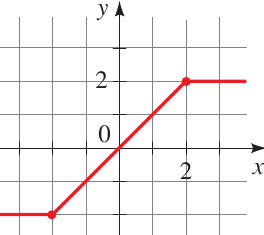
\includegraphics[width=0.48\textwidth]{fig_p02_49.png}\end{center}

\begin{paso}{Paso 1 --- Tramo izquierdo}
\textbf{Qué hago:} leo la altura del trozo horizontal de la izquierda.

\textbf{¿De dónde sale?} De la gráfica: para $x<-2$ el trazo es horizontal a la altura $-2$.

\textbf{¿Por qué?} Un segmento horizontal es la gráfica de una función constante $f(x)=b$, con $b$ la altura leída: $f(x)=-2$.
\end{paso}

\begin{paso}{Paso 2 --- Tramo central}
\textbf{Qué hago:} calculo la recta que pasa por los extremos $(-2,-2)$ y $(2,2)$.

\textbf{¿De dónde sale?} De la gráfica, el trozo oblicuo va de $(-2,-2)$ a $(2,2)$; su pendiente es $m=\dfrac{2-(-2)}{2-(-2)}=\dfrac{4}{4}=1$ y pasa por el origen.

\textbf{¿Por qué?} Una función lineal $f(x)=mx+b$ tiene gráfica recta; con $m=1$ y punto de intersección $b=0$ queda $f(x)=x$.
\end{paso}

\begin{paso}{Paso 3 --- Tramo derecho}
\textbf{Qué hago:} leo la altura del trozo horizontal de la derecha.

\textbf{¿De dónde sale?} De la gráfica: a partir de $(2,2)$ el trazo es horizontal a la altura $2$.

\textbf{¿Por qué?} Otra vez un segmento horizontal es una constante: $f(x)=2$.
\end{paso}

\begin{resp}
\[
f(x)=\begin{cases}-2 & \text{si } x<-2\\ x & \text{si } -2<x\le 2\\ 2 & \text{si } x>2\end{cases}
\]
\end{resp}

\begin{nota}
El molde impreso del libro no cubre $x=-2$ (dice $x<-2$ y luego $-2<x\le 2$). En la gráfica el punto $(-2,-2)$ aparece sólido y ambas fórmulas dan $-2$ ahí, así que el valor es $f(-2)=-2$ con cualquiera de las dos convenciones; es una omisión del enunciado, no una ambigüedad de la gráfica.
\end{nota}

% =====================================================================
\subsection*{Ejercicio 10 — Prueba de la recta vertical (Ej.~51, p.~168)}

\begin{quote}
\textbf{51--52} $\blacksquare$ \textbf{Prueba de la recta vertical} \quad Use la prueba de la recta vertical para determinar si la curva es la gráfica de una función de $x$.

\textbf{51.} \quad \textit{a}) \hspace{4.2cm} \textit{b})
\end{quote}

\begin{center}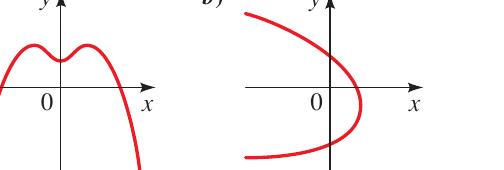
\includegraphics[width=0.62\textwidth]{fig_p02_51.png}\end{center}

\begin{paso}{Paso 1 --- Inciso \textit{a}}
\textbf{Qué hago:} deslizo mentalmente rectas verticales sobre la curva de dos jorobas.

\textbf{¿De dónde sale?} De la figura: la curva sube, baja un poco, vuelve a subir y luego cae, pero nunca se devuelve hacia la izquierda.

\textbf{¿Por qué?} Ninguna recta vertical la corta más de una vez, así que por la prueba de la recta vertical sí es la gráfica de una función de $x$.
\end{paso}

\begin{paso}{Paso 2 --- Inciso \textit{b}}
\textbf{Qué hago:} traslado una vertical sobre la curva acostada en forma de C.

\textbf{¿De dónde sale?} De la figura: para cada $x$ a la izquierda del punto más a la derecha hay una rama arriba y otra abajo.

\textbf{¿Por qué?} Esa vertical corta la curva dos veces, en $(a,b)$ y en $(a,c)$ con $b\ne c$, y una función no puede asignar dos valores distintos a la misma entrada: no es gráfica de una función de $x$.
\end{paso}

\begin{resp}
\textit{a}) Sí es la gráfica de una función de $x$. \quad \textit{b}) No lo es.
\end{resp}

% =====================================================================
\subsection*{Ejercicio 11 — Recta vertical, dominio y rango (Ej.~55, p.~168)}

\begin{quote}
\textbf{53--56} $\blacksquare$ \textbf{Prueba de la recta vertical: dominio y rango} \quad Use la prueba de la recta vertical para determinar si la curva es la gráfica de una función de $x$. Si lo es indique el dominio y el rango de la función.

\textbf{55.}
\end{quote}

\begin{center}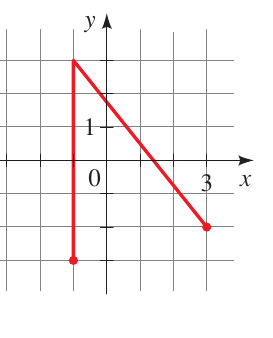
\includegraphics[width=0.42\textwidth]{fig_p02_55.png}\end{center}

\begin{paso}{Paso 1 --- Identifico el trozo vertical}
\textbf{Qué hago:} localizo el segmento rojo que sube verticalmente en $x=-1$.

\textbf{¿De dónde sale?} De la figura: en $x=-1$ el trazo va desde $y=-3$ hasta $y=3$ antes de que arranque el segmento inclinado hacia $(3,-2)$.

\textbf{¿Por qué?} Ese trozo es literalmente parte de una recta vertical, así que la vertical $x=-1$ coincide con la curva en infinitos puntos, no en uno solo.
\end{paso}

\begin{paso}{Paso 2 --- Aplico la prueba}
\textbf{Qué hago:} concluyo con la prueba de la recta vertical.

\textbf{¿De dónde sale?} Del paso 1: la recta $x=-1$ corta la curva más de una vez.

\textbf{¿Por qué?} La prueba dice que una curva es gráfica de una función si y sólo si ninguna vertical la corta más de una vez; aquí falla, así que la curva no define $y$ como función de $x$ y no procede dar dominio ni rango.
\end{paso}

\begin{resp}
No es la gráfica de una función de $x$: la recta vertical $x=-1$ corta la curva en todo el segmento de $y=-3$ a $y=3$. Por eso el enunciado no pide dominio ni rango en este caso.
\end{resp}

% =====================================================================
\subsection*{Ejercicio 12 — ¿$3x-5y=7$ define una función? (Ej.~57, p.~168)}

\begin{quote}
\textbf{57--68} $\blacksquare$ \textbf{Ecuaciones que definen funciones} \quad Determine si la ecuación define a $y$ como función de $x$. (Vea el ejemplo 9.)

\textbf{57.} $3x-5y=7$
\end{quote}

\begin{paso}{Paso 1 --- Despejo $y$}
\textbf{Qué hago:} aíslo $y$ pasando $3x$ y dividiendo entre $-5$.

\textbf{¿De dónde sale?} De la ecuación $3x-5y=7$ del enunciado.

\textbf{¿Por qué?} El criterio del ejemplo 9 es despejar $y$ en términos de $x$ y ver cuántos valores resultan.

\[
3x-5y=7 \;\Longrightarrow\; -5y=7-3x \;\Longrightarrow\; y=\frac{3x-7}{5}.
\]
\end{paso}

\begin{paso}{Paso 2 --- Cuento las salidas}
\textbf{Qué hago:} observo que la expresión final no tiene $\pm$ ni raíces pares.

\textbf{¿De dónde sale?} Del despeje: $y=\dfrac{3x-7}{5}$ es una operación aritmética única sobre $x$.

\textbf{¿Por qué?} Cada $x$ produce exactamente un $y$, que es la definición de función; en notación de funciones, $f(x)=\dfrac{3x-7}{5}$, una función lineal.
\end{paso}

\begin{resp}
Sí define a $y$ como función de $x$: $\;f(x)=\dfrac{3x-7}{5}=\dfrac{3}{5}x-\dfrac{7}{5}$.
\end{resp}

% =====================================================================
\subsection*{Ejercicio 13 — ¿$2x-4y^2=3$ define una función? (Ej.~61, p.~168)}

\begin{quote}
\textbf{61.} $2x-4y^2=3$
\end{quote}

\begin{paso}{Paso 1 --- Despejo $y^2$}
\textbf{Qué hago:} aíslo el término con $y$ y divido entre $-4$.

\textbf{¿De dónde sale?} De $2x-4y^2=3$: paso $2x$ al otro lado y obtengo $-4y^2=3-2x$.

\textbf{¿Por qué?} Igual que en el ejemplo 9\textit{b}, el primer objetivo es dejar $y$ sola.

\[
-4y^2=3-2x \;\Longrightarrow\; y^2=\frac{2x-3}{4}.
\]
\end{paso}

\begin{paso}{Paso 2 --- Tomo raíces cuadradas}
\textbf{Qué hago:} extraigo raíz cuadrada en ambos lados, con signo $\pm$.

\textbf{¿De dónde sale?} De $y^2=\dfrac{2x-3}{4}$ del paso 1.

\textbf{¿Por qué?} Si $y^2=k$ con $k>0$ hay dos soluciones, $y=+\sqrt{k}$ y $y=-\sqrt{k}$, porque ambas elevadas al cuadrado dan $k$.

\[
y=\pm\sqrt{\frac{2x-3}{4}}=\pm\frac{\sqrt{2x-3}}{2}.
\]
\end{paso}

\begin{paso}{Paso 3 --- Contraejemplo concreto}
\textbf{Qué hago:} exhibo una entrada con dos salidas.

\textbf{¿De dónde sale?} Con $x=\tfrac72$: $y^2=\dfrac{2(7/2)-3}{4}=\dfrac{4}{4}=1$, luego $y=1$ y $y=-1$.

\textbf{¿Por qué?} Una función asigna a cada entrada exactamente una salida; aquí $x=\tfrac72$ tiene dos, así que la ecuación no define a $y$ como función de $x$.
\end{paso}

\begin{resp}
No define a $y$ como función de $x$: el despeje da $y=\pm\dfrac{\sqrt{2x-3}}{2}$, dos valores de $y$ para cada $x>\tfrac32$.
\end{resp}

% =====================================================================
\subsection*{Ejercicio 14 — Tarifas de una empresa eléctrica (Ej.~81, p.~169)}

\begin{quote}
\textbf{81. Tarifas de una empresa} \quad La empresa Westside Energy cobra a sus consumidores de energía eléctrica una tarifa base de 6.00 dólares por mes, más 10 centavos por kilowatt-hora (kWh) por los primeros 300 kWh consumidos y 6 centavos por kWh por el consumo mayor de 300 kWh. Suponga que un cliente usa $x$ kWh de electricidad en un mes.

\quad \textit{a}) Exprese el costo mensual $E$ como una función de $x$ definida por tramos.

\quad \textit{b}) Trace la gráfica de la función $E$ para $0\le x\le 600$.
\end{quote}

\begin{paso}{Paso 1 --- Primer tramo: hasta 300 kWh}
\textbf{Qué hago:} escribo el costo cuando $0\le x\le 300$.

\textbf{¿De dónde sale?} Del enunciado: base de $6.00$ dólares más $10$ centavos $=0.10$ dólares por cada uno de los $x$ kWh.

\textbf{¿Por qué?} El cargo variable es proporcional al consumo, así que se suma $0.10x$ a la base fija.

\[
E(x)=6+0.10x \qquad \text{si } 0\le x\le 300.
\]
\end{paso}

\begin{paso}{Paso 2 --- Segundo tramo: más de 300 kWh}
\textbf{Qué hago:} cobro los primeros $300$ kWh a la tarifa alta y el excedente $x-300$ a $0.06$.

\textbf{¿De dónde sale?} Los primeros $300$ kWh cuestan $0.10(300)=30$; sumados a la base dan $6+30=36$. El excedente son $x-300$ kWh a $0.06$ cada uno.

\textbf{¿Por qué?} La tarifa de $6$ centavos se aplica sólo al consumo \emph{mayor} de $300$ kWh, no a todo el consumo.

\[
E(x)=36+0.06(x-300)=18+0.06x \qquad \text{si } x>300.
\]
\end{paso}

\begin{paso}{Paso 3 --- Verifico el empalme y trazo}
\textbf{Qué hago:} comparo las dos fórmulas en $x=300$ y evalúo en $x=600$.

\textbf{¿De dónde sale?} $6+0.10(300)=36$ y $18+0.06(300)=36$; además $E(600)=18+0.06(600)=54$.

\textbf{¿Por qué?} Coinciden en la frontera, así que la gráfica es continua: dos segmentos de recta unidos en $(300,36)$, el segundo menos inclinado porque su pendiente $0.06$ es menor que $0.10$.

\begin{center}
\begin{tikzpicture}
\begin{axis}[axis lines=left,xlabel=$x$ (kWh),ylabel=$E$ (dólares),xmin=0,xmax=640,ymin=0,ymax=60,
 width=11cm,height=6cm,xtick={0,100,200,300,400,500,600},ytick={6,36,54}]
\addplot[thick,red,domain=0:300]{6+0.1*x};
\addplot[thick,red,domain=300:600]{18+0.06*x};
\addplot[only marks,mark=*,red,mark size=1.6pt] coordinates {(0,6)(300,36)(600,54)};
\end{axis}
\end{tikzpicture}
\end{center}
\end{paso}

\begin{resp}
\[
E(x)=\begin{cases}6+0.10x & \text{si } 0\le x\le 300\\ 18+0.06x & \text{si } x>300\end{cases}
\]
Gráfica: segmento de $(0,6)$ a $(300,36)$ y segmento de $(300,36)$ a $(600,54)$.
\end{resp}

% =====================================================================
\subsection*{Ejercicio 15 — Tarifas postales (Ej.~83, p.~169)}

\begin{quote}
\textbf{83. Tarifas postales} \quad La tarifa nacional de costos de envío postal por cartas de primera clase, de 3.5 onzas o menos, es de 49 centavos por la primera onza (o menos), más 21 centavos por cada onza adicional (o parte de una onza). Exprese el costo de envío postal $P$ como una función definida por tramos del peso $x$ de una carta, con $0<x\le 3.5$, y trace la gráfica de esta función.
\end{quote}

\begin{paso}{Paso 1 --- Cuento onzas empezadas}
\textbf{Qué hago:} identifico los intervalos de peso que pagan lo mismo.

\textbf{¿De dónde sale?} Del enunciado: se cobra por onza \emph{o parte de una onza}, así que una carta de $1.3$ oz paga igual que una de $2$ oz.

\textbf{¿Por qué?} El cargo depende del número de onzas empezadas, no del peso exacto: los intervalos son $(0,1]$, $(1,2]$, $(2,3]$ y $(3,3.5]$.
\end{paso}

\begin{paso}{Paso 2 --- Calculo el costo de cada intervalo}
\textbf{Qué hago:} sumo $0.49$ por la primera onza y $0.21$ por cada onza adicional empezada.

\textbf{¿De dónde sale?} $0.49$; $0.49+0.21=0.70$; $0.49+2(0.21)=0.91$; $0.49+3(0.21)=1.12$.

\textbf{¿Por qué?} En cada intervalo la carta tiene una onza adicional empezada más que en el anterior, y cada una cuesta $0.21$ dólares.
\end{paso}

\begin{paso}{Paso 3 --- Escribo la función y la trazo}
\textbf{Qué hago:} armo los cuatro tramos y dibujo los segmentos horizontales.

\textbf{¿De dónde sale?} De los intervalos del paso 1 con los costos del paso 2.

\textbf{¿Por qué?} Es una función escalón: constante en cada intervalo, con salto de $0.21$ al pasar de uno al siguiente. El extremo derecho de cada tramo es sólido (se incluye) y el izquierdo hueco.

\begin{center}
\begin{tikzpicture}
\begin{axis}[axis lines=left,xlabel=$x$ (onzas),ylabel=$P$ (dólares),xmin=0,xmax=4,ymin=0,ymax=1.35,
 width=10.5cm,height=6cm,xtick={0,1,2,3,3.5},ytick={0.49,0.70,0.91,1.12},yticklabels={$0{,}49$,$0{,}70$,$0{,}91$,$1{,}12$}]
\addplot[thick,red,domain=0:1]{0.49};
\addplot[thick,red,domain=1:2]{0.70};
\addplot[thick,red,domain=2:3]{0.91};
\addplot[thick,red,domain=3:3.5]{1.12};
\addplot[only marks,mark=*,red,mark size=2pt] coordinates {(1,0.49)(2,0.70)(3,0.91)(3.5,1.12)};
\addplot[only marks,mark=o,red,thick,mark size=2pt] coordinates {(0,0.49)(1,0.70)(2,0.91)(3,1.12)};
\end{axis}
\end{tikzpicture}
\end{center}
\end{paso}

\begin{resp}
\[
P(x)=\begin{cases}
0.49 & \text{si } 0<x\le 1\\
0.70 & \text{si } 1<x\le 2\\
0.91 & \text{si } 2<x\le 3\\
1.12 & \text{si } 3<x\le 3.5
\end{cases}
\]
(en dólares). La gráfica es una escalera de cuatro peldaños horizontales, con salto de $0.21$ en $x=1,2,3$.
\end{resp}

\end{document}
